\documentclass[conference]{IEEEtran}
\IEEEoverridecommandlockouts
% The preceding line is only needed to identify funding in the first footnote. If that is unneeded, please comment it out.
\usepackage{cite}
\usepackage{amsmath,amssymb,amsfonts}
\usepackage{algorithmic}
\usepackage{graphicx}
\usepackage{textcomp}
\usepackage{xcolor}
\usepackage{placeins}
\usepackage{float}
\usepackage{stfloats} % permite figure* con [b] (doble columna abajo); se carga después de float
\usepackage{url}
\renewcommand{\abstractname}{Resumen}
\renewcommand{\refname}{Referencias}
\renewcommand{\IEEEkeywordsname}{Palabras claves}
\def\BibTeX{{\rm B\kern-.05em{\sc i\kern-.025em b}\kern-.08em
    T\kern-.1667em\lower.7ex\hbox{E}\kern-.125emX}}

% Ajustes de separación y parámetros de flotantes
\setlength{\textfloatsep}{6pt plus 2pt minus 2pt}
\setlength{\dbltextfloatsep}{6pt plus 2pt minus 2pt}
\setlength{\intextsep}{6pt plus 2pt minus 2pt}
\renewcommand{\dblfloatpagefraction}{0.8}
\renewcommand{\dbltopfraction}{0.9}
\renewcommand{\bottomfraction}{0.9}
\renewcommand{\textfraction}{0.1}
\renewcommand{\topfraction}{0.9}
\renewcommand{\floatpagefraction}{0.8}

% Salto de fila entre autores, con cada fila centrada
\makeatletter
\newcommand{\linebreakand}{%
  \end{@IEEEauthorhalign}
  \hfill\mbox{}\par
  \mbox{}\hfill\begin{@IEEEauthorhalign}
}
\makeatother

\begin{document}

\title{Detección de ataques de red multiclase sobre UNSW-NB15: análisis exploratorio y evaluación de modelos de Machine Learning}

\author{\IEEEauthorblockN{1\textsuperscript{st} Fabricio Alonso Lanche Pacsi}
\IEEEauthorblockA{\textit{dept. Computación} \\
\textit{Ciencias de la Computación}\\
Lima, Perú \\
fabricio.lanche@utec.edu.pe}
\and
\IEEEauthorblockN{2\textsuperscript{nd} Jhogan Haldo Pachacutec Aguilar}
\IEEEauthorblockA{\textit{dept. Computación} \\
\textit{Ciencias de la Computación}\\
Lima, Perú\\
jhogan.pachacutec@utec.edu.pe}
\and
\IEEEauthorblockN{3\textsuperscript{rd} Anyeli Azumi Tamara Ureta}
\IEEEauthorblockA{\textit{dept. Computación} \\
\textit{Ciencias de la Computación}\\
Lima, Perú \\
anyeli.tamara@utec.edu.pe}
\linebreakand
\IEEEauthorblockN{4\textsuperscript{th} Paulo Isael Miranda Barrientos}
\IEEEauthorblockA{\textit{dept. Computación} \\
\textit{Ciencias de la Computación}\\
Lima, Perú \\
paulo.miranda@utec.edu.pe}
\and
\IEEEauthorblockN{5\textsuperscript{th} Christopher Renato Perez Torres}
\IEEEauthorblockA{\textit{dept. Computación} \\
\textit{Ciencias de Datos}\\
Lima, Perú \\
christopher.perez@utec.edu.pe}
}

\maketitle

\begin{abstract}
Este proyecto analiza el dataset UNSW-NB15 para desarrollar y evaluar modelos de Machine Learning capaces de clasificar tráfico de red en distintas categorías de ataques, considerando el desbalance de clases, la calidad de los datos y las características más relevantes para la detección de intrusiones.
\end{abstract}

\begin{IEEEkeywords}
UNSW-NB15, clasificación, ciberseguridad, EDA.
\end{IEEEkeywords}

\subsection{Motivación y relevancia del problema}

La detección de intrusiones en redes constituye un problema relevante en ciberseguridad por la frecuencia y diversidad de las amenazas actuales. Según el \textit{ENISA Threat Landscape 2025} \cite{enisa2025}, los ataques DDoS representaron aproximadamente el 77\,\% de los incidentes reportados, mientras que el ransomware destacó por su impacto. Además, el phishing estuvo involucrado en el 60\,\% de los puntos iniciales de intrusión, seguido por la explotación de vulnerabilidades con un 21,3\,\%. Estas cifras reflejan que las amenazas difieren tanto en sus mecanismos como en sus consecuencias, por lo que detectarlas no solo implica distinguir el tráfico benigno del malicioso, sino también identificar qué tipo de ataque se está produciendo.

En este contexto, la clasificación multiclase permite caracterizar con mayor precisión los flujos maliciosos y aportar información útil para analizar los incidentes y orientar la respuesta. Para estudiar esta tarea se utilizará el dataset \textbf{UNSW-NB15}, cuyos registros describen las características y el comportamiento de conexiones de red. En particular, se empleará \texttt{attack\_cat} como variable objetivo, que identifica el tráfico benigno y nueve familias de ataques.

\subsection{Formulación del problema y objetivo de ML}

El problema consiste en clasificar los flujos de tráfico de red según su naturaleza y, en particular, identificar la familia a la que pertenece cada ataque, en lugar de limitarse a distinguir entre tráfico benigno y malicioso. Esta tarea requiere aprender patrones de comunicación que permitan diferenciar comportamientos de ataque y generalizar a flujos no observados durante el entrenamiento, con el propósito de aportar información útil para el análisis de incidentes de seguridad.

Para ello, se empleará aprendizaje supervisado sobre el dataset UNSW-NB15, que proporciona etiquetas de referencia (\textit{ground truth}) en la variable \texttt{attack\_cat} \cite{moustafa2015unsw}. El objetivo es entrenar un modelo de clasificación multiclase que asigne cada flujo a una de diez categorías, correspondientes al tráfico normal (\texttt{Benign}) y a nueve familias de ataques cibernéticos: \texttt{Generic}, \texttt{Exploits}, \texttt{Fuzzers}, \texttt{DoS}, \texttt{Reconnaissance}, \texttt{Analysis}, \texttt{Backdoors}, \texttt{Shellcode} y \texttt{Worms} \cite{moustafa2016evaluation}.

\subsection{Preguntas de investigación}

\textbf{Pregunta de investigación principal:}

¿En qué medida las características de los flujos de tráfico de red del dataset UNSW-NB15 permiten clasificar correctamente cada registro como una de las distintas categorías de ataque mediante técnicas de Machine Learning?

\textbf{Preguntas de investigación específicas:}

\begin{itemize}
    \item ¿Qué características del tráfico de red presentan mayor relación con la categoría de ataque identificada por \texttt{attack\_cat}?
    
    \item ¿Existen categorías de tráfico que presenten patrones similares y, por lo tanto, sean más difíciles de distinguir entre sí?
    
    \item ¿Cómo influye la distribución de las clases en la capacidad de identificar correctamente las distintas categorías de tráfico?
\end{itemize}
\FloatBarrier

\section{Datos y Análisis Exploratorio de Datos (EDA)}

Esta sección presenta el análisis exploratorio del proyecto. Los scripts y el código necesarios para reproducir el análisis se encuentran disponibles en el repositorio del proyecto \cite{repo}.

\subsection{Descripción del dataset}

El dataset UNSW-NB15 \cite{moustafa2015unsw} fue generado en el Cyber Range Lab de la ACCS, combinando tráfico normal real con ataques sintéticos de IXIA PerfectStorm, con el fin de superar las limitaciones de KDD99 y NSL-KDD \cite{moustafa2016evaluation}. Contiene 2\,540\,044 flujos bidireccionales distribuidos en cuatro archivos CSV y 49 columnas, extraídas con Argus, Bro-IDS y doce algoritmos adicionales. En este trabajo se emplea la versión completa de Kaggle \cite{kaggle_unsw} en lugar de la partición reducida de 175\,341 y 82\,332 registros publicada por los autores \cite{moustafa2016evaluation}, de modo que las clases minoritarias queden mejor representadas.

\subsection{Variables y variable objetivo}

Las 49 columnas se distribuyen en cinco grupos de variables y dos etiquetas (Tabla~\ref{tab:grupos_variables}). Las variables de flujo (5) identifican la conexión mediante IP, puertos y protocolo, mientras que las básicas (13) describen propiedades como duración, bytes y TTL; las de contenido (8) registran información de cabeceras TCP y transacciones HTTP, y las temporales (9) caracterizan variaciones como el \textit{jitter} y los tiempos de \textit{handshake}. Por último, las adicionales (12) contabilizan patrones en ventanas de hasta 100 flujos, como combinaciones repetidas de IP, puerto o servicio, útiles para detectar escaneos y ráfagas. En conjunto, hay 41 variables numéricas y varias nominales, entre ellas algunas de alta cardinalidad (\texttt{srcip}, \texttt{dstip}, \texttt{sport}, \texttt{dsport}) y otras de baja (\texttt{proto}, \texttt{state}, \texttt{service}) \cite{moustafa2016evaluation}.

\begin{table}[H]
\centering
\caption{Grupos de variables del dataset UNSW-NB15 (Moustafa \& 
Slay, 2016).}
\label{tab:grupos_variables}
\footnotesize
\begin{tabular}{@{}p{1.6cm}p{0.7cm}p{4.3cm}@{}}
\hline
\textbf{Grupo} & \textbf{N.} & \textbf{Ejemplos} \\
\hline
Flujo & 5 & srcip, dstip, sport, proto \\
Básicas & 13 & state, dur, sbytes, sttl \\
Contenido & 8 & swin, smeansz, trans\_depth \\
Tiempo & 9 & sjit, sintpkt, tcprtt \\
Adicionales & 12 & ct\_state\_ttl, ct\_srv\_src \\
\hline
Etiquetas & 2 & attack\_cat, label \\
\hline
\textbf{Total} & \textbf{49} & \\
\hline
\end{tabular}
\end{table}

El dataset incluye \texttt{label}, que distingue tráfico normal (0) de ataques (1), y \texttt{attack\_cat}, que identifica la categoría específica. Se adopta esta última como variable objetivo, con \texttt{Benign} como clase legítima y nueve familias de ataque que completan las diez clases. Estas abarcan desde intentos de provocar fallos mediante datos malformados (\texttt{Fuzzers}) y la explotación de vulnerabilidades (\texttt{Exploits}), hasta la saturación de recursos (\texttt{DoS}) y el acceso remoto no autorizado mediante puertas traseras (\texttt{Backdoors}). Otras categorías comprenden el sondeo de redes para identificar objetivos (\texttt{Reconnaissance}), el análisis de servicios y aplicaciones (\texttt{Analysis}), los ataques genéricos basados en técnicas comunes (\texttt{Generic}), la ejecución de código malicioso (\texttt{Shellcode}) y la propagación de malware autorreplicable (\texttt{Worms}).

% [CAMBIO] Bloque de figuras adelantado (antes estaba tras «Variables y variable objetivo»).
% Fig. 1 -> parte superior de su página; Fig. 2 -> parte inferior de la misma página.
% Fig. 1 se declara primero para conservar la numeración.
\begin{figure*}[!t]
\centering
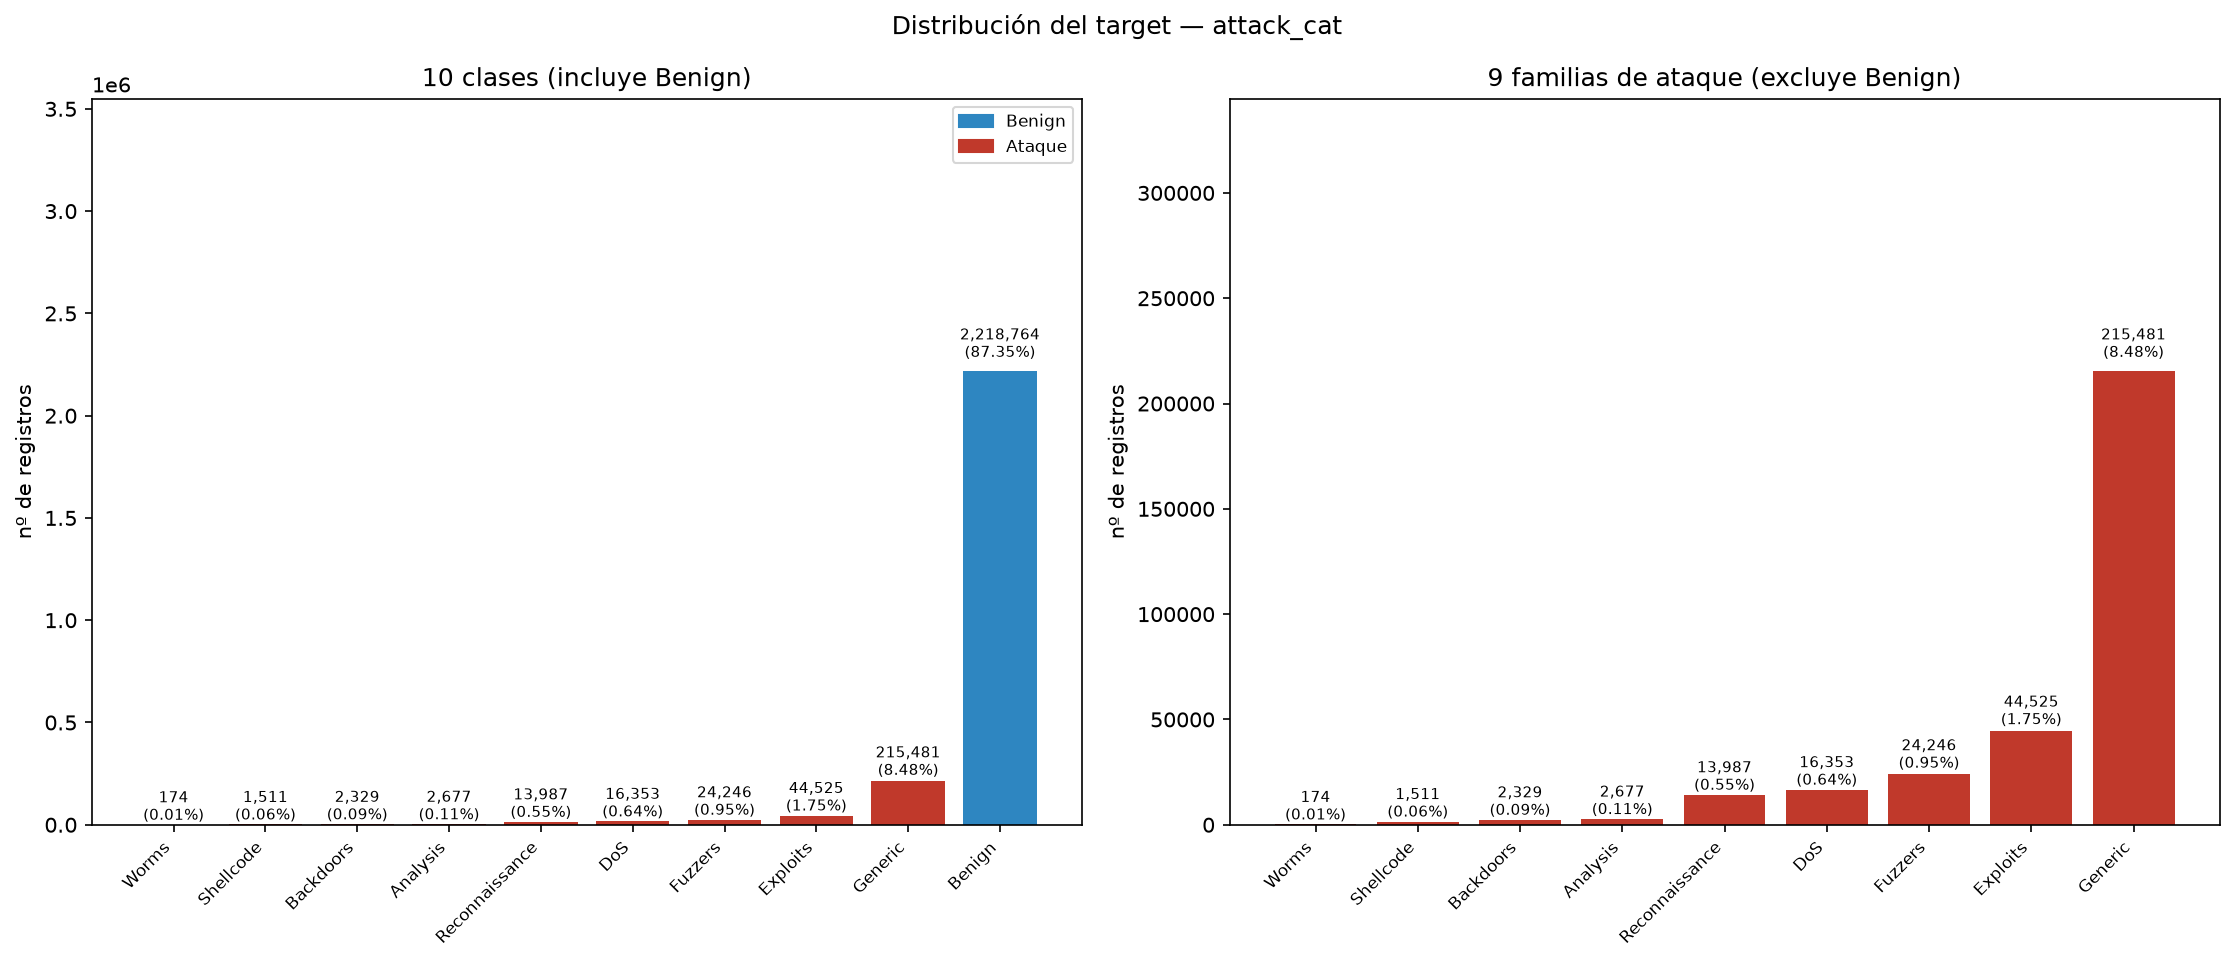
\includegraphics[width=0.7\textwidth,keepaspectratio]{output/fig01_distribucion_clases.png}
\caption{Distribución de \texttt{attack\_cat}: las diez clases (izquierda) y las nueve familias de ataque sin \texttt{Benign} (derecha).}
\label{fig:clases}
\end{figure*}

\begin{figure*}[!b]
\centering
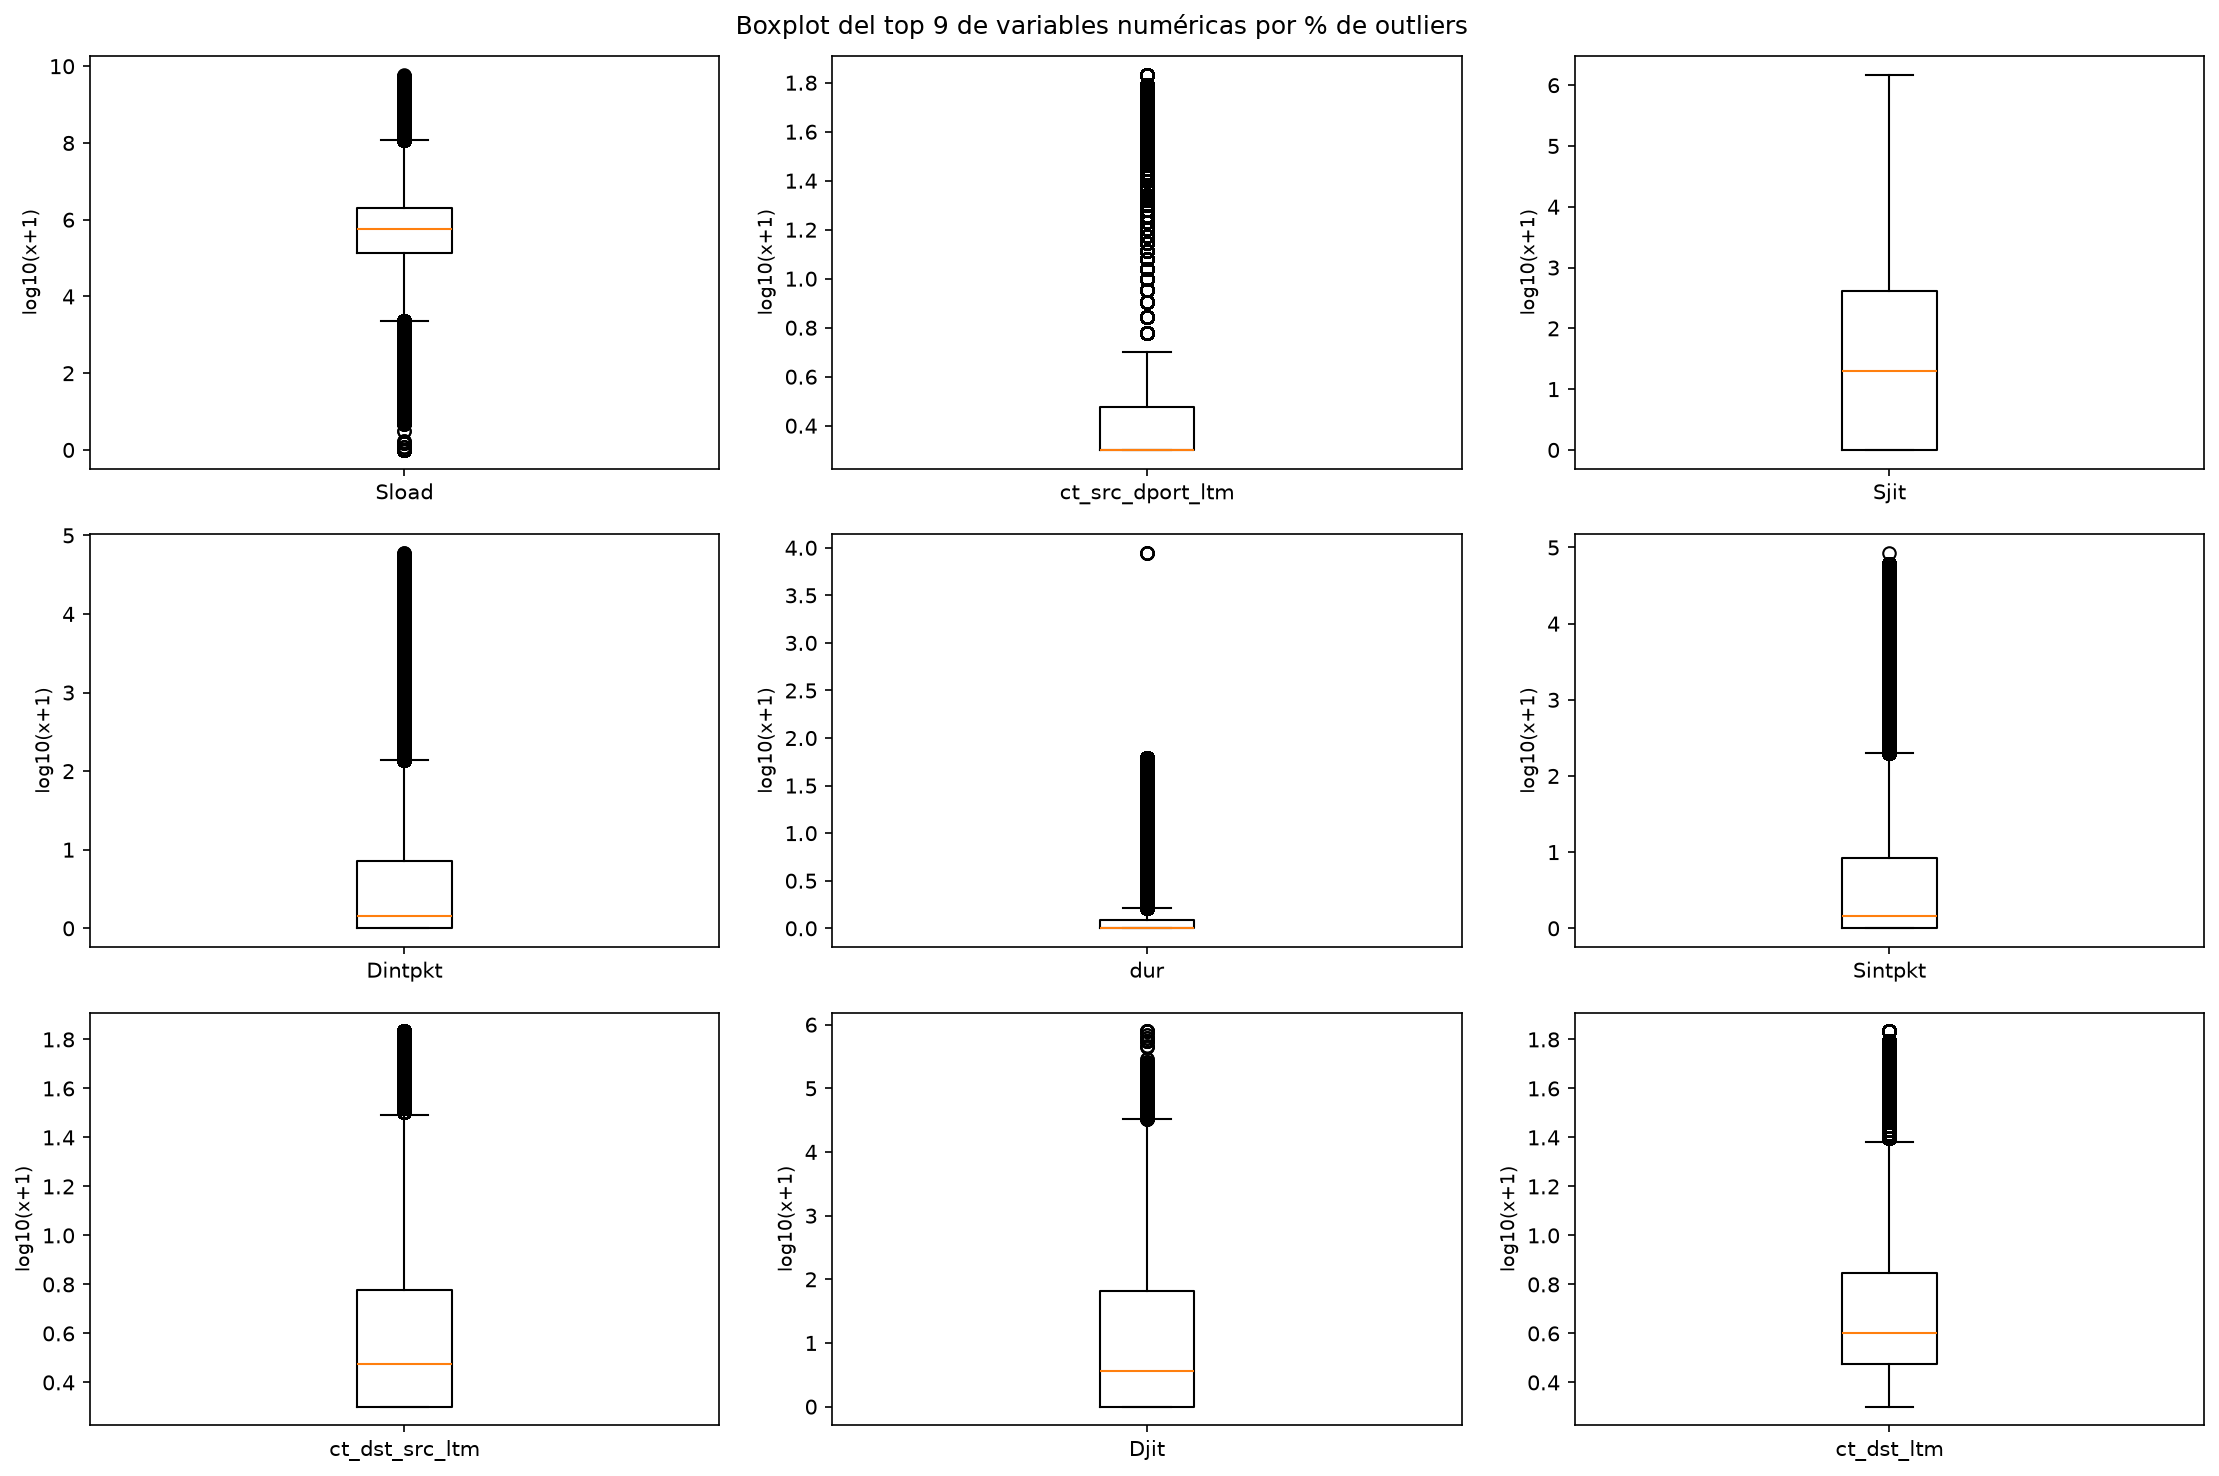
\includegraphics[width=0.7\textwidth,keepaspectratio]{output/fig02_boxplot_outliers.png}
\caption{Boxplots en escala logarítmica de una selección de variables numéricas. Los puntos fuera de los bigotes corresponden a valores atípicos según el criterio IQR.}
\label{fig:boxplot}
\end{figure*}

\subsection{Valores faltantes}

El 57.20\,\% de los registros presenta al menos un valor ausente, concentrado en seis de las 49 columnas (Tabla~\ref{tab:faltantes}). La mayoría son ausencias estructurales: \texttt{is\_ftp\_login} y \texttt{ct\_ftp\_cmd} solo aplican a sesiones FTP y \texttt{ct\_flw\_http\_mthd} a sesiones HTTP, por lo que su ausencia indica que la variable no aplica al flujo, no un fallo de captura. Los demás faltantes afectan a \texttt{sport} (8), \texttt{dsport} (304) y \texttt{state} (8), un total de 320 filas (menos del 0.02\,\%), y provienen de tokens corruptos en la fuente original, como literales hexadecimales ilegibles y la cadena "\texttt{no}" en \texttt{state}.

Los faltantes tampoco se distribuyen uniformemente entre los archivos de origen. Para \texttt{is\_ftp\_login}, el archivo 1 no presenta blancos, mientras que los archivos 3 y 4 superan el 98\,\%; además, aparecen en el 57.69\,\% del tráfico no FTP y en el 37.39\,\% del FTP. Esto sugiere que la codificación de la ausencia refleja, al menos parcialmente, la procedencia del registro y no solo el protocolo del flujo.


\begin{table}[H]
\centering
\caption{Valores faltantes por columna.}
\label{tab:faltantes}
\footnotesize
\begin{tabular}{lrrl}
\hline
\textbf{Columna} & \textbf{Faltantes} & \textbf{\%} & \textbf{Origen} \\
\hline
\texttt{is\_ftp\_login} & 1,430,065 & 56.30 & FTP \\
\texttt{ct\_ftp\_cmd}    & 1,429,879 & 56.29 & FTP \\
\texttt{ct\_flw\_http\_mthd} & 1,348,145 & 53.08 & HTTP \\
\texttt{dsport}          & 304       & 0.01  & Token \\
\texttt{sport}           & 8         & 0.00  & Token \\
\texttt{state}           & 8         & 0.00  & Token \\
\hline
\end{tabular}
\end{table}

\subsection{Distribución de variables y clases}

La variable objetivo \texttt{attack\_cat} define una tarea de clasificación multiclase con diez categorías, correspondientes a nueve familias de ataque y la clase legítima \texttt{Benign}. La Fig.~\ref{fig:clases} muestra un desbalance marcado entre ellas. El 87.35\,\% de los registros corresponde a \texttt{Benign}, mientras que \texttt{Generic} concentra 215\,481 observaciones (8.48\,\%) y \texttt{Worms} apenas 174. Esto implica que un modelo puede obtener un buen desempeño global favoreciendo las clases mayoritarias, por lo que la evaluación debe reportar el rendimiento por categoría.

La Tabla~\ref{tab:descriptivos} resume los estadísticos de una selección de variables numéricas pertenecientes a distintos grupos funcionales. Varias presentan asimetrías pronunciadas, con medias muy superiores a sus medianas, como \texttt{Sjit} (1\,589 frente a 19.12) y \texttt{Sintpkt} (193.32 frente a 0.47). Esto indica que las variables no comparten escala ni distribución y que sus valores extremos pueden dominar ciertas representaciones numéricas.

\begin{table}[!tb]
\centering
\caption{Estadísticos descriptivos de variables numéricas seleccionadas por grupo funcional.}
\label{tab:descriptivos}
\footnotesize
\resizebox{\columnwidth}{!}{%
\begin{tabular}{llrrrrr}
\hline
\textbf{Grupo} & \textbf{Variable} & \textbf{Media} & \textbf{Mediana} & \textbf{Varianza} & \textbf{Mín} & \textbf{Máx} \\
\hline
Básicas & \texttt{dur} & 0.66 & 0.02 & 193.90 & 0.00 & 8,787 \\
Básicas & \texttt{sbytes} & 4,340 & 1,470 & 3.182e+09 & 0.00 & 1.436e+07 \\
Básicas & \texttt{sttl} & 62.78 & 31.00 & 5,569 & 0.00 & 255.00 \\
Contenido & \texttt{trans\_depth} & 0.08 & 0.00 & 0.12 & 0.00 & 172.00 \\
Tiempo & \texttt{Sjit} & 1,589 & 19.12 & 2.860e+08 & 0.00 & 1,483,831 \\
Tiempo & \texttt{Sintpkt} & 193.32 & 0.47 & 7,723,748 & 0.00 & 84,371 \\
Adicionales & \texttt{ct\_state\_ttl} & 0.26 & 0.00 & 0.47 & 0.00 & 6.00 \\
Adicionales & \texttt{ct\_srv\_src} & 9.21 & 5.00 & 117.44 & 1.00 & 67.00 \\
\hline
\end{tabular}}
\end{table}

\subsection{Problemas de calidad y outliers}

Además de los faltantes, se identificaron 480\,633 filas duplicadas equivalentes al 18.92\,\% del total. Estos duplicados se concentran especialmente en \texttt{Generic} (88.22\,\%), \texttt{DoS} (65.36\,\%) y \texttt{Exploits} (38.01\,\%), frente al 11.67\,\% de \texttt{Benign}. Esta distribución es consistente con el carácter sintético de varias familias de ataque, cuyos flujos pueden repetirse de forma idéntica en ráfagas, mientras que el tráfico benigno presenta mayor diversidad. Por tanto, la duplicación afecta de forma desigual a las clases, puede reforzar artificialmente ciertos patrones y sobreestimar el desempeño si observaciones idénticas aparecen tanto en entrenamiento como en prueba.

La cardinalidad de las variables nominales también revela particularidades del escenario de captura. Las direcciones \texttt{srcip} y \texttt{dstip} presentan apenas 43 y 47 valores únicos, respectivamente, lo que apunta a una diversidad limitada de hosts. En cambio, \texttt{sport} y \texttt{dsport} alcanzan 64\,598 y 64\,627 valores únicos, mientras que \texttt{proto}, \texttt{state} y \texttt{service} contienen solo 135, 16 y 13 categorías. Esta combinación puede llevar a los modelos a asociar las clases con hosts o puertos específicos en lugar de con el comportamiento de los ataques, limitando su generalización a otras redes.

En las variables numéricas, los valores atípicos se concentran en distribuciones de cola larga, especialmente en \texttt{Sload} (22.17\,\% de outliers según el criterio IQR), \texttt{ct\_src\_dport\_ltm} (21.01\,\%), \texttt{Sjit} (18.63\,\%), \texttt{Dintpkt} (17.86\,\%), \texttt{dur} (17.77\,\%) y \texttt{Sintpkt} (17.56\,\%). Por otro lado, algunas variables presentan una proporción elevada de ceros, como \texttt{ct\_ftp\_cmd} (96.07\,\%), \texttt{res\_bdy\_len} (92.65\,\%) y \texttt{trans\_depth} (91.92\,\%), debido a que sus métricas solo aplican a determinados tipos de conexión. La Fig.~\ref{fig:boxplot} muestra, en escala logarítmica, la dispersión de variables representativas sin que los valores extremos oculten las magnitudes menores. Las colas largas y los valores concentrados en cero deberán considerarse en el preprocesamiento, pues afectan de forma distinta a las transformaciones y a los modelos.

% [CAMBIO] Se eliminó el \FloatBarrier que estaba aquí (causaba la columna vacía)

\subsection{Relaciones entre variables (correlaciones)}

La asociación con el objetivo se evaluó con dos medidas complementarias. Frente al target binario, la correlación de Pearson sitúa a \texttt{sttl} como el predictor más asociado (0.90), seguido de \texttt{Dload} (-0.22); el resto presenta valores débiles o moderados. Como el problema es multiclase, esta medida es solo orientativa: la razón de correlación $\eta^2$, estimada sobre una muestra de 500\,000 registros, cuantifica la proporción de varianza de cada variable numérica explicada por las diez clases,
\begin{equation}
    \eta^{2} = \frac{\mathrm{SSB}}{\mathrm{SST}} = \frac{\sum_{g} n_{g}(\bar{y}_{g} - \bar{y})^{2}}{\sum_{i} (y_{i} - \bar{y})^{2}},
\end{equation}
donde $\bar{y}_{g}$ y $n_{g}$ son la media y el número de observaciones de la clase $g$, y $\bar{y}$ es la media global. La Tabla~\ref{tab:eta} resume los diez valores más altos: \texttt{sttl} (0.835) y \texttt{ct\_state\_ttl} (0.777) encabezan la discriminación, seguidos por los contadores \texttt{ct\_*} (0.22--0.32); el resto no supera 0.14, de modo que la capacidad discriminativa se concentra en pocas variables.

% [CAMBIO] Tabla fijada con [H]: aparece primero, justo tras el párrafo que la cita
\begin{table}[H]
\centering
\caption{Razón de correlación $\eta^2$ entre las variables numéricas y \texttt{attack\_cat} (diez valores más altos).}
\label{tab:eta}
\footnotesize
\resizebox{\columnwidth}{!}{%
\begin{tabular}{lrlr}
\hline
\textbf{Variable} & \textbf{$\eta^2$} & \textbf{Variable} & \textbf{$\eta^2$} \\
\hline
\texttt{sttl} & 0.835 & \texttt{ct\_srv\_dst} & 0.290 \\
\texttt{ct\_state\_ttl} & 0.777 & \texttt{ct\_srv\_src} & 0.283 \\
\texttt{ct\_dst\_src\_ltm} & 0.324 & \texttt{ct\_src\_dport\_ltm} & 0.274 \\
\texttt{dttl} & 0.307 & \texttt{ct\_dst\_ltm} & 0.238 \\
\texttt{ct\_dst\_sport\_ltm} & 0.301 & \texttt{ct\_src\_ltm} & 0.226 \\
\hline
\end{tabular}}
\end{table}


La Fig.~\ref{fig:correlacion} reúne las asociaciones entre predictores y target, así como las relaciones de redundancia entre variables. Entre los contadores, \texttt{ct\_state\_ttl} (0.874) y \texttt{ct\_dst\_src\_ltm} (0.440) son los más asociados con el target. Sin embargo, esta señal puede reflejar tanto el comportamiento de los ataques como la repetición de flujos en las ráfagas capturadas. Al recalcular $\eta^2$ sin duplicados, \texttt{ct\_state\_ttl} disminuye de 0.78 a 0.50 y \texttt{ct\_srv\_src} cae de 0.28 a 0.12, lo que sugiere que parte de la capacidad discriminativa de los contadores depende de la composición de las ráfagas y no solo de patrones propios de cada clase.

% [CAMBIO] [!tb] -> [!b]: la figura solo puede ir al pie, nunca encima de la tabla
\begin{figure}[!b]
\centering
\includegraphics[width=\columnwidth,trim=10 10 10 10,clip]{output/fig03_correlacion_seleccion.png}
\caption{Matriz de correlación de Pearson entre variables seleccionadas y el target binario.}
\label{fig:correlacion}
\end{figure}


La matriz también evidencia redundancia entre predictores. Las correlaciones entre \texttt{Stime} y \texttt{Ltime} (1.00), \texttt{swin} y \texttt{dwin} (0.997), y \texttt{sbytes} y \texttt{sloss} (0.954) indican que estos pares contienen información prácticamente equivalente, y se observan asociaciones elevadas incluso entre variables de grupos distintos, como \texttt{sttl} y \texttt{ct\_state\_ttl} (0.906), y entre \texttt{ct\_dst\_src\_ltm} y \texttt{ct\_srv\_src} (0.942). Junto con la baja capacidad discriminativa de varias variables, esto indica que incorporar más atributos no necesariamente aporta información nueva, lo que motiva examinar la contribución individual de los predictores y reducir redundancias durante el preprocesamiento.



\subsection{Sesgo y data leakage}

El análisis exploratorio muestra que el dataset presenta características que condicionan la comparación entre modelos. Existe un marcado desbalance de clases: el 87.35\,\% de los registros corresponde a tráfico \texttt{Benign}, mientras que \texttt{Worms} cuenta con apenas 174 observaciones. Por ello, la exactitud global resulta insuficiente y es necesario considerar métricas desagregadas por clase. La presencia de duplicados implica un compromiso entre preservar la representación de las familias de ataque y evitar una sobreestimación del desempeño. Conservarlos mantendría la distribución original, mientras que eliminarlos elevaría \texttt{Benign} al 95.16\,\%. Sin embargo, conservarlos también puede inflar las métricas al contabilizar varias veces un mismo flujo.

El origen controlado de la captura introduce otros sesgos que pueden limitar la generalización. Las direcciones IP presentan apenas 43 y 47 valores distintos, mientras que los puertos rondan los 64\,000, lo que puede facilitar asociaciones entre hosts, puertos y clases que difícilmente se mantendrían en una red real. Las variables numéricas presentan colas largas y numerosos valores atípicos, especialmente en \texttt{Sload}, \texttt{Sjit} y \texttt{dur} (Fig.~\ref{fig:boxplot}). También existe redundancia entre variables, con correlaciones de 1.00 entre \texttt{Stime} y \texttt{Ltime}, de 0.997 entre \texttt{swin} y \texttt{dwin}, y de 0.96 entre \texttt{sbytes} y \texttt{sloss}. Asimismo, la capacidad discriminativa se concentra en pocas variables: solo \texttt{sttl} y \texttt{ct\_state\_ttl} alcanzan una razón $\eta^2$ superior a 0.7, mientras que otras variables \texttt{ct\_*} y \texttt{dttl} presentan valores entre 0.22 y 0.32 (Tabla~\ref{tab:eta}). En conjunto, el aprendizaje puede depender de un subconjunto reducido de variables y de patrones específicos de la captura, en lugar de reflejar características generalizables del tráfico.

La fuga de información constituye un problema distinto, pues puede producir estimaciones que no reflejan la capacidad real de generalización. \texttt{attack\_cat} y \texttt{label} codifican la misma información, por lo que incluirlas como entradas permitiría acceder directamente a la respuesta. De forma similar, las direcciones IP, los puertos sin transformar y \texttt{Stime}/\texttt{Ltime} pueden inducir asociaciones espurias al reflejar la identidad de los hosts o el instante de captura. Las variables \texttt{ct\_*} requieren un matiz adicional: al contabilizar conexiones en ventanas de 100 flujos que incluyen la observación actual, pueden calcularse al cierre de cada conexión sin recurrir necesariamente a información futura. El riesgo reside en la partición, pues si una misma ráfaga aparece en entrenamiento y prueba, el modelo podría aprender su composición en lugar de reconocer patrones generalizables de los ataques. Los duplicados exactos agravan este problema bajo una partición aleatoria, pues una misma observación puede aparecer en ambos conjuntos y favorecer una sobreestimación del desempeño.


\section{Preprocesamiento e ingeniería de características}
\section{Metodología y modelos}

\subsection{Formulación del aprendizaje y justificación del enfoque}
La detección de intrusiones en red se aborda bajo el paradigma de aprendizaje supervisado. Al disponer del conjunto de datos UNSW-NB15 etiquetado mediante la variable objetivo \texttt{attack\_cat}, los modelos se optimizan para aprender los patrones de tráfico (duración de flujo, conteo de paquetes, protocolos y marcas de tiempo) y asociarlos explícitamente con sus clases correspondientes \cite{moustafa2015unsw, moustafa2016evaluation}. Se descarta un enfoque no supervisado (\textit{clustering}) dado que el objetivo del proyecto no es descubrir estructuras anómalas a ciegas, sino entrenar clasificadores capaces de discriminar con precisión entre tráfico normal y 9 familias de ataques cibernéticos específicas.

\subsection{Selección de modelos de aprendizaje}
Para evaluar la discriminación del tráfico de red, se seleccionan clasificadores de distinta naturaleza estructural, siguiendo precedentes en la literatura sobre UNSW-NB15 \cite{more2024enhanced}:
\begin{enumerate}
    \item \textbf{Regresión Logística Multinomial (Baseline):} Clasificador lineal que sirve como referencia base para evaluar el sesgo de linealidad en los datos.
    \item \textbf{Máquina de Vectores de Soporte (SVM):} Modelo no lineal orientado a la maximización del margen de separación en espacios de alta dimensión.
    \item \textbf{Random Forest:} Método de ensamble basado en \textit{Bagging} (\textit{Bootstrap Aggregating}) que combina múltiples árboles de decisión, reduciendo varianza y capturando interacciones complejas entre predictores.
\end{enumerate}

\section{Diseño experimental y evaluación}
\section{Resultados y análisis}
\section{Discusión y limitaciones}
\section{Conclusiones}

\begin{thebibliography}{00}
\bibitem{kaggle_unsw}
H. Bhangale,
``UNSW Complete Dataset,''
\textit{Kaggle}, 2023. [Online]. Available:
https://www.kaggle.com/datasets/harshwardhanbhangale/unsw-complete-dataset

\bibitem{enisa2025}
European Union Agency for Cybersecurity (ENISA),
``ENISA Threat Landscape 2025,''
2025. [Online]. Available:
https://www.enisa.europa.eu/publications/enisa-threat-landscape-2025

\bibitem{kaufman2012leakage}
S. Kaufman, S. Rosset, C. Perlich, and O. Stitelman,
``Leakage in data mining: Formulation, detection, and avoidance,''
\textit{ACM Transactions on Knowledge Discovery from Data (TKDD)},
vol. 6, no. 4, pp. 1--21, 2012.

\bibitem{repo}
F. A. Lanche Pacsi et al.,
``ml-project,''
GitHub, 2026. [Online]. Available:
\url{https://github.com/FabricioLanche/ml-project}

\bibitem{mehrabi2021survey}
N. Mehrabi, F. Morstatter, N. Saxena, K. Lerman, and A. Galstyan,
``A survey on bias and fairness in machine learning,''
\textit{ACM Computing Surveys (CSUR)},
vol. 54, no. 6, pp. 1--35, 2021.

\bibitem{more2024enhanced}
S. More, M. Idrissi, H. Mahmoud, and A. T. Asyhari,
``Enhanced Intrusion Detection Systems Performance with UNSW-NB15 Data Analysis,''
\textit{Algorithms},
vol. 17, no. 2, p. 64, 2024, doi: 10.3390/a17020064.

\bibitem{moustafa2015unsw}
N. Moustafa and J. Slay,
``UNSW-NB15: A comprehensive data set for network intrusion detection systems (UNSW-NB15 network data set),''
in \textit{2015 Military Communications and Information Systems Conference (MilCIS)},
Canberra, Australia, 2015, pp. 1--6.

\bibitem{moustafa2016evaluation}
N. Moustafa and J. Slay,
``The evaluation of Network Anomaly Detection Systems: Statistical analysis of the UNSW-NB15 data set and the comparison with the KDD99 data set,''
\textit{Information Security Journal: A Global Perspective},
vol. 25, no. 1--3, pp. 18--31, 2016.

\end{thebibliography}
\end{document}